\section{Stratifying $M$}

Stratifying $\RR$ via the singular values of $f$ also induces a stratification of $M$
by considering the fibers of $f$ above the stratifying regions.
The interiors of face regions have preimage through $f$ a disjoint collection of face blocks, the interiors of edge regions have preimage of edge blocks, and of vertex regions, vertex blocks.

To understand the structure of face, edge, and vertex blocks we investigate the preimages of regular and singular values of $f$ in the plane.
\begin{defn}
	Because $M$ is closed, $f$ is proper.
	Thus, for any point $q$ in $f(M)$, a fiber of $f$ above $q$ (i.e.\ a connected component of $f\inv(q)$) is either a closed 1--manifold (i.e.\ $S^1$) or contains a critical point of $f$.
	
	We define a \emph{singular fiber} to be a fiber that contains a critical point of $f$, and a \emph{regular fiber} to be a fiber consisting entirely of regular points.	
\end{defn}

The subsets used to stratify $M$ are the fibers of $f$ that lie above the corners of the octagonal vertex regions, the edges of the vertex and edge regions, and the regions themselves.
Because the corners of the vertex regions are regular values, their fibers are regular, hence a finite collection of disjointly embedded circles in $M$.
We take these circles as the first collection of subsets that filter $M$, and assign to them the indices $(1,i)$ for $i = 1\dots N_1$, where $N_1$ is the number of circles.
These circles are disjoint, so $(1,i)\nleq (1,j)$ for any $i,j$.

The arcs of the $\RR$ stratification connect the vertices of the $\RR$ stratification and either consist entirely of regular values or contain exactly one singular value.
As pictured in Figure \ref{fig:face-sleeve}, an arc contains exactly one singular value precisely when it is the boundary a vertex region and an edge region.
When an arc contains exactly one singular value, exactly one fiber above that value is a singular fiber, with the rest regular fibers.
A decomposing arc is diffeomorphic to the unit interval and $f$ is a smooth submersion between smooth manifolds, so a fiber above a decomposing arc is a surface whose boundary circles are the fibers above the arc's endpoints.
When the fiber is regular, the surface is diffeomorphic to an annulus $S^1\times\Ilit$.
When the fiber is singular, the surface classification depends on the type of singularity.
Theorem \ref{thm:saeki} and Figure \ref{fig:saeki-fibers} show that the fiber containing the singularity either has the structure of a figure-of-eight (when the singularity is part of an indefinite fold) or is a single point (when the singularity is part of a definite fold), hence the singular fiber above the arc is diffeomorphic to either a 2--disk or a pair-of-pants.

Theorem \ref{thm:saeki} refers to a \emph{stable map}, and we'll denote the set of smooth stable maps $X\to Y$ by $Stab(X,Y)$.
When $X$ is a smooth, closed, orientable 3--manifold and $Y$ is the plane, $Stab(X,Y)$ consists of all maps $X\to Y$ satisfying the first five stratification conditions.
The last stratification condition is trivially satisfied because $X$ is closed, hence the set of stratifying maps $X\to Y$ is the subset of $Stab(X,Y)$ consisting of maps $f$ such that $f(S(f))$ is connected.

\begin{theorem}[Adapted Theorem 3.15 in Saeki \cite{Saeki}]
	\label{thm:saeki}
	Let $f:M\to N$ be a proper $C^\infty$ stable map of an orientable 3--manifold $M$ into a surface $N$.
	Then, every singular fiber of $f$ is equivalent to the disjoint union of:
	\begin{enumerate}
		\item one of the fibers in Figure \ref{fig:saeki-fibers}, and
		\item the disjoint union of a finite number of copies of $S^1$.
	\end{enumerate}
	Furthermore, no two fibers in the list are equivalent to each other even after taking the union with regular circle components.		
\end{theorem}

\begin{figure}[h!]
	\centering
	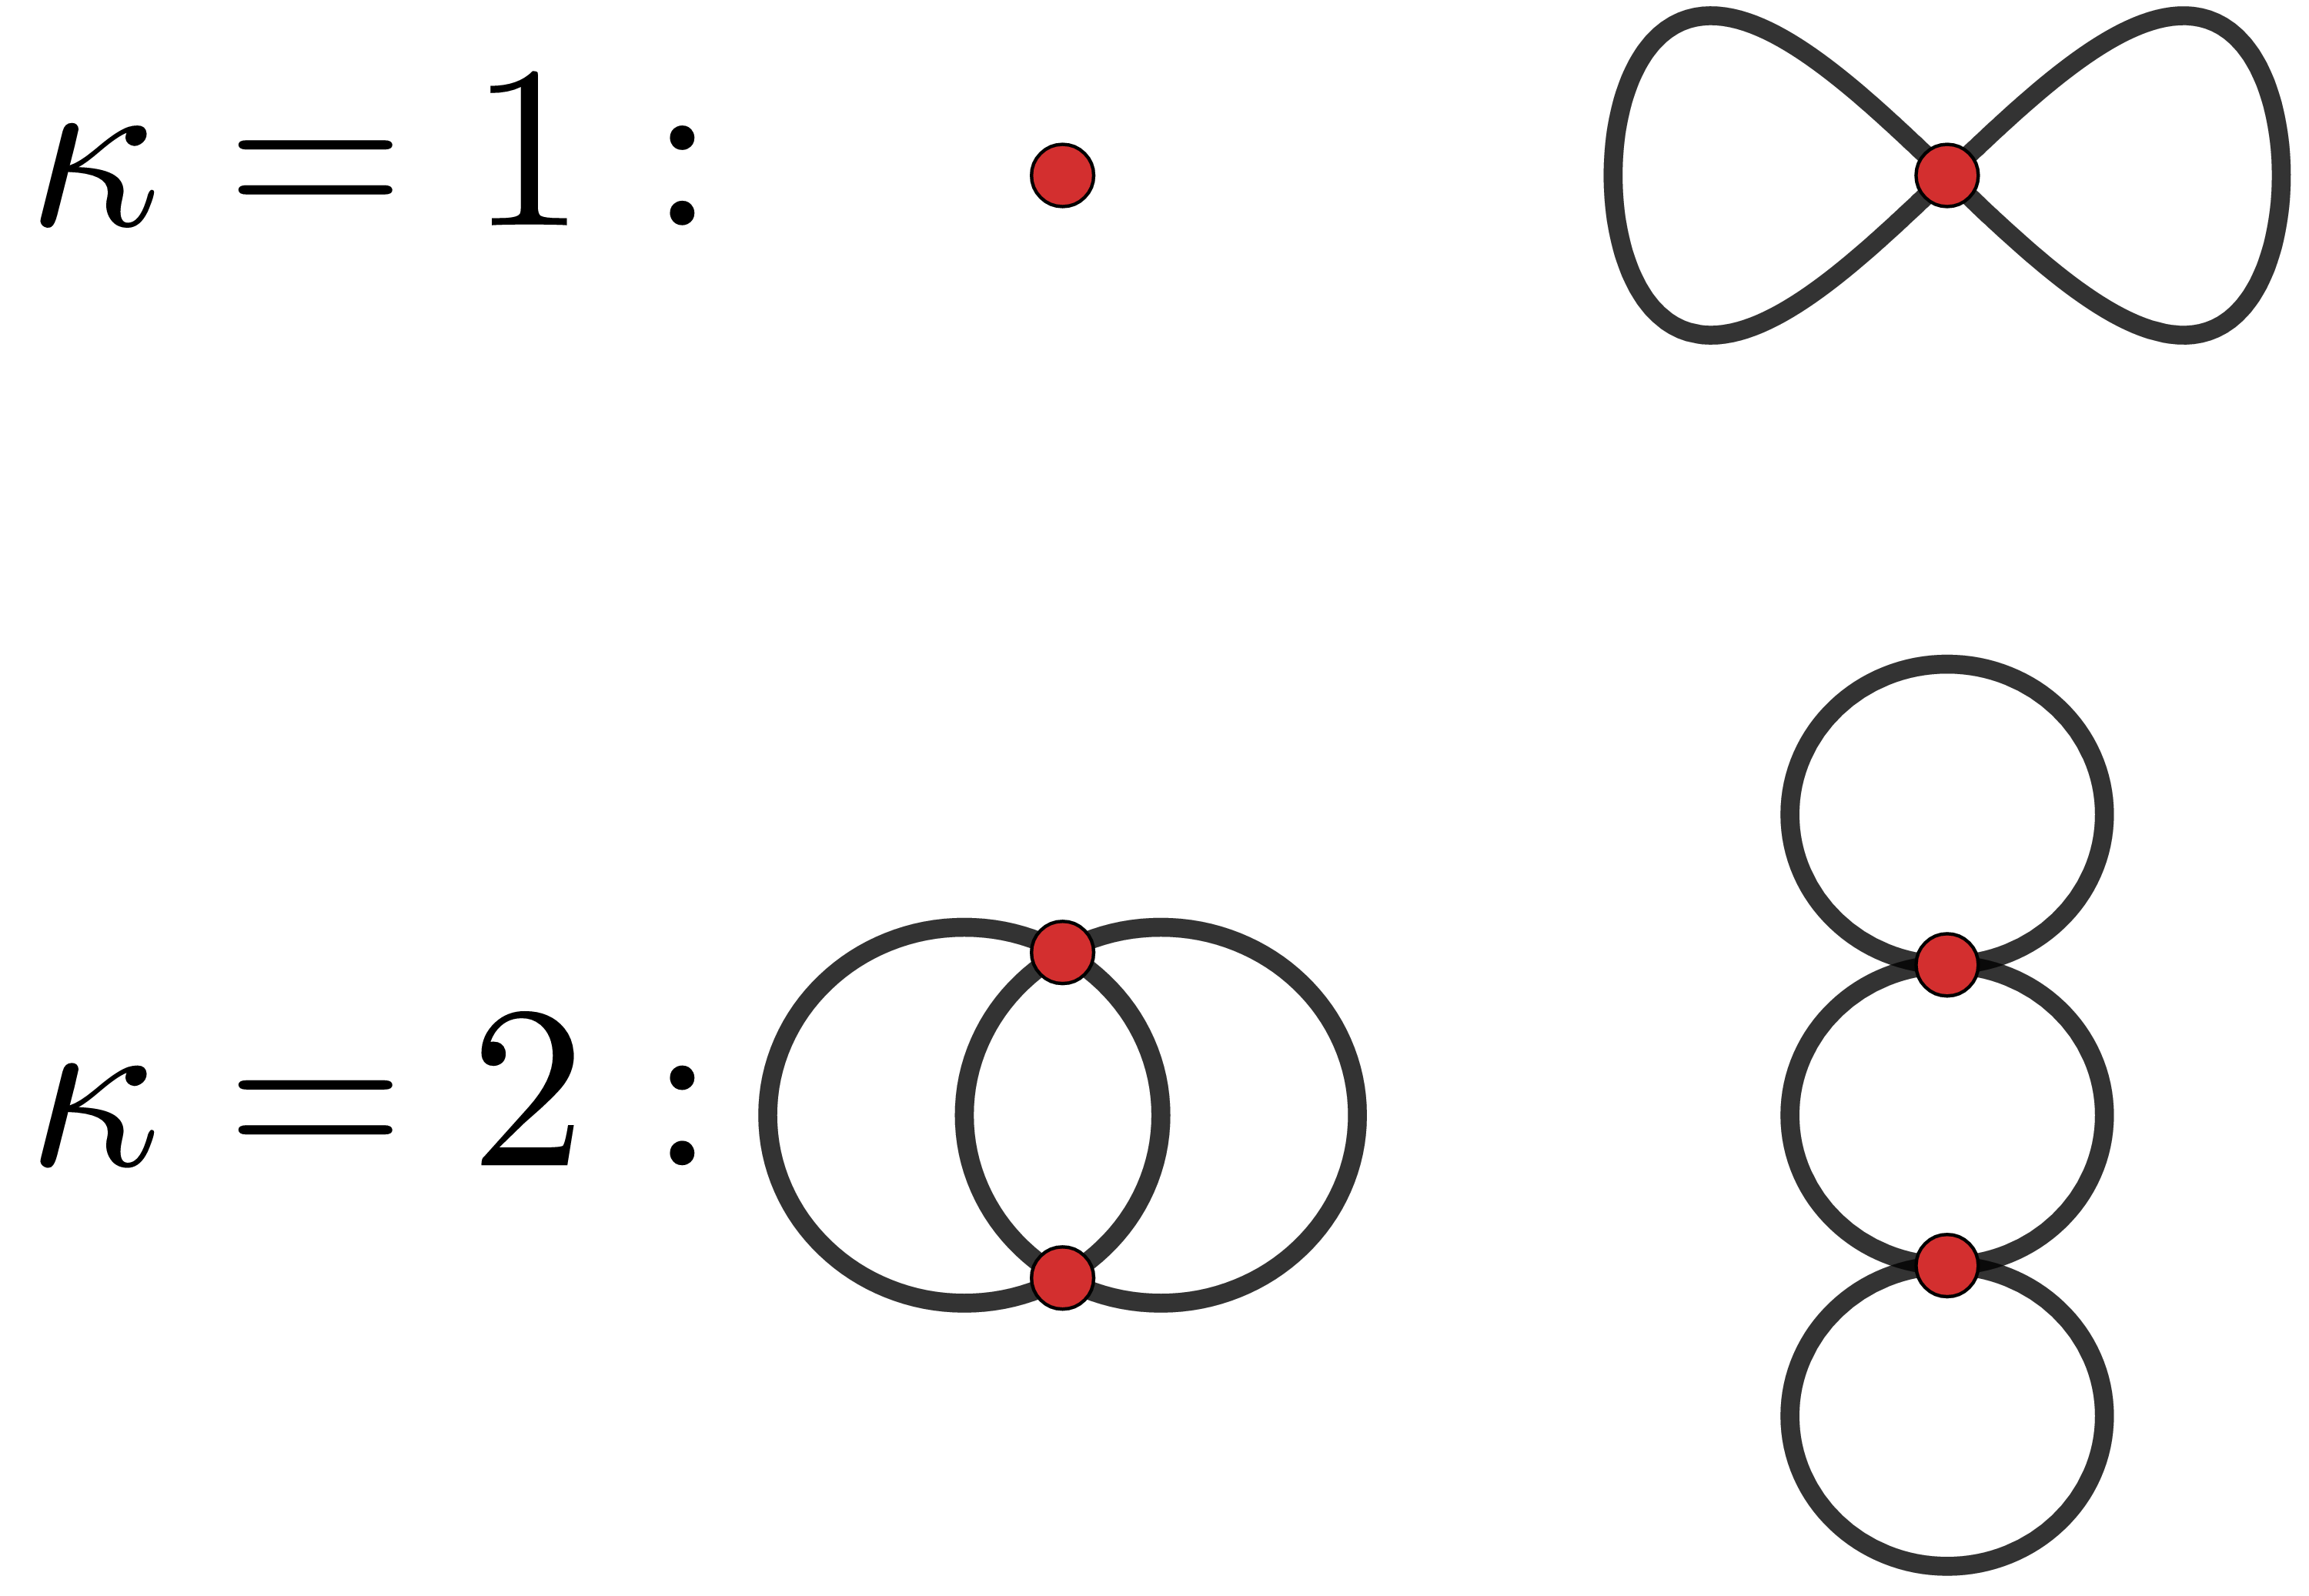
\includegraphics{figures/saeki-fibers.png}
	\caption{
		\textbf{Connected singular fibers.}
		List of connected singular fibers of proper $C^\infty$ stable maps of orientable 3--manifolds into surfaces.
		$\kappa$ is the codimension of the singularity in the surface.
		The singular fiber above a codimension 2 singular value may be disconnected,
		in which case the fiber is the disjoint union of a pair of singular fibers from $\kappa=1$.
	}
	\label{fig:saeki-fibers}	
\end{figure}

The surface fibers above the decomposing arcs are the second collection of subsets that filter $M$, and they are assigned the indices $(2,j)$ for $j=1\dots N_2$, where $N_2$ is the number of surfaces.
The boundary circles of the surfaces are each subsets of the filtration, indexed by the $(1,i)$ indices, so $(1,i)\leq (2,j)$ if and only if $M_{(1,i)}$ is one of the boundary components of $M_{(2,j)}$.
These surfaces intersect one another only when they share a boundary circle, so $(2,j)\nleq (2,k)$ for any $j,k$.

There are three types of region in the decomposition: face, edge, and vertex.
Regardless of the type of region, they are indexed in our filtration similarly to the edges.
A fiber above a region is a 3--manifold with corners formed by the $(1,i)$- and $(2,j)$-level strata, and fibers are disjoint away from their boundaries.
We therefore index fibers above regions with the indices $(3,k)$ for $k=1\dots N_3$ where $N_3$ is the total number of fibers above regions, put $(n,i)\leq (3,k)$ if and only if $M_{(n,i)}$ is contained in the boundary of $M_{(3,k)}$.

Recall that we call a closed 3--dimensional stratum of $M$ a \emph{block}.
We now restate the desired block structure laid out at the beginning of this chapter and prove that the stratification conditions impose this structure on the blocks of $M$.

\begin{theorem}
	\label{thm:block-structure}
	Let $M$ be a smooth, closed, orientable 3--manifold, let $f:M\to\RR$ be a stratifying map, suppose $\RR$ has been decomposed as in Section \ref{section:smooth-decompose} and $M$ has been stratified as in this section.
	Then each closed strata $M_{(3,k)}$ is classified as either a \emph{face}, \emph{edge}, or \emph{vertex block} depending on whether it is a fiber above a face, edge, or vertex region respectively, and a block has one of the following structures:
	\begin{itemize}
		\item \emph{face block}:
		Let $B$ be a face block that fibers over the face region $F$.
		Then $B$ is stratified--homeomorphic to $S^1\times F$.
		
		\item \emph{edge block}:
		Let $B$ be an edge block that fibers over the edge region $E$.
		Let $A$ be the annulus $S^1\times\Ilit$ and $P$ the pair-of pants surface (i.e.\ $D^2$ minus a pair of disjoint open balls).
		If $B$ is a regular fiber over $E$ then $B$ is stratified--homeomorphic to $S^1\times E$, hence also stratified--homeomorphic to $A\times\Ilit$.
		Otherwise, $B$ is a singular fiber over $E$ and contains part of definite or indefinite fold.
		In this case we call $B$ a \emph{definite} or \emph{indefinite edge block}.
		A definite edge block is stratified--homeomorphic to $D^2\times\Ilit$ and an indefinite edge block is stratified--homeomorphic to $P\times\Ilit$.

		\item \emph{vertex block}:
		Let $B$ be a vertex block that fibers over the vertex region $V$.
		If $B$ is a regular fiber then it is homeomorphic to $S^1\times V$, therefore homeomorphic to a (3,1)--handlebody of genus 1.
		Otherwise, we see from Figure \ref{fig:saeki-fibers} that the singular fiber above the codimension 2 singularity contained in $V$ is either connected or disconnected.
		If the singular fiber is disconnected then there are a pair of disjoint vertex blocks that each contain one of the singular fibers, hence part of a definite or indefinite fold.
		We therefore classify these blocks as \emph{definite} or \emph{indefinite vertex blocks}.
		If the singular fiber is connected, then the block containing it is an \emph{interactive vertex block}.
		A definite (resp.\ indefinite) vertex block extends and connects definite (resp.\ indefinite) edge blocks, and is homeomorphic to a (3,1)--handlebody of genus 0 (resp.\ 2).
		An interactive vertex block is homeomorphic to a (3,1)--handlebody of genus 3.
	\end{itemize}
\end{theorem}

\begin{rmk}
	The structures of the blocks described in Theorem \ref{thm:block-structure} are roughly disk bundles over a representative fiber for the given region or, equivalently, regular neighbourhoods of that fiber.
	For a block that is a regular fiber, the representative is a circle.
	For a definite or indefinite block, the representative is the singular fiber containing a definite or indefinite fold, and for an interactive block the representative fiber is the singular fiber above the codimension 2 singular value.
\end{rmk}

\begin{proof}[Proof of Theorem \ref{thm:block-structure}]
	We split the proof into three parts.
	The first part proves that if a block $B$ is a regular fiber over the region $R$ then $B$ is stratified--homeomorphic to $S^1\times R$.
	In the second part, we prove that definite and indefinite blocks are stratified--homeomorphic to $D^2\times\Ilit$ or $P\times\Ilit$ respectively.
	In the final part we discuss interactive vertex blocks, and show that they are homeomorphic to (3,1)--handlebodies of genus 3.
	Figures illustrate the block structures.
	
	\textbf{Part 1:}
	Let $B$ be a block over the region $R$, and suppose $B$ consists entirely of regular fibers over $R$.
	Then $(B, R, f|_B, S^1)$ has the structure of a circle bundle over $R$.
	A fiber bundle over a contractible space is trivial, so $B$ is homeomorphic to $S^1 \times R$.
	Furthermore, this homeomorphism is stratified by ensuring the strata of $B$ are mapped to the strata of $S^1 \times R$, where the stratification of $S^1 \times R$ is defined by the manifold with corners structure induced by the product topology.
	See Figure \ref{fig:regular-blocks}.
	
	\begin{figure}[h]
		\centering
		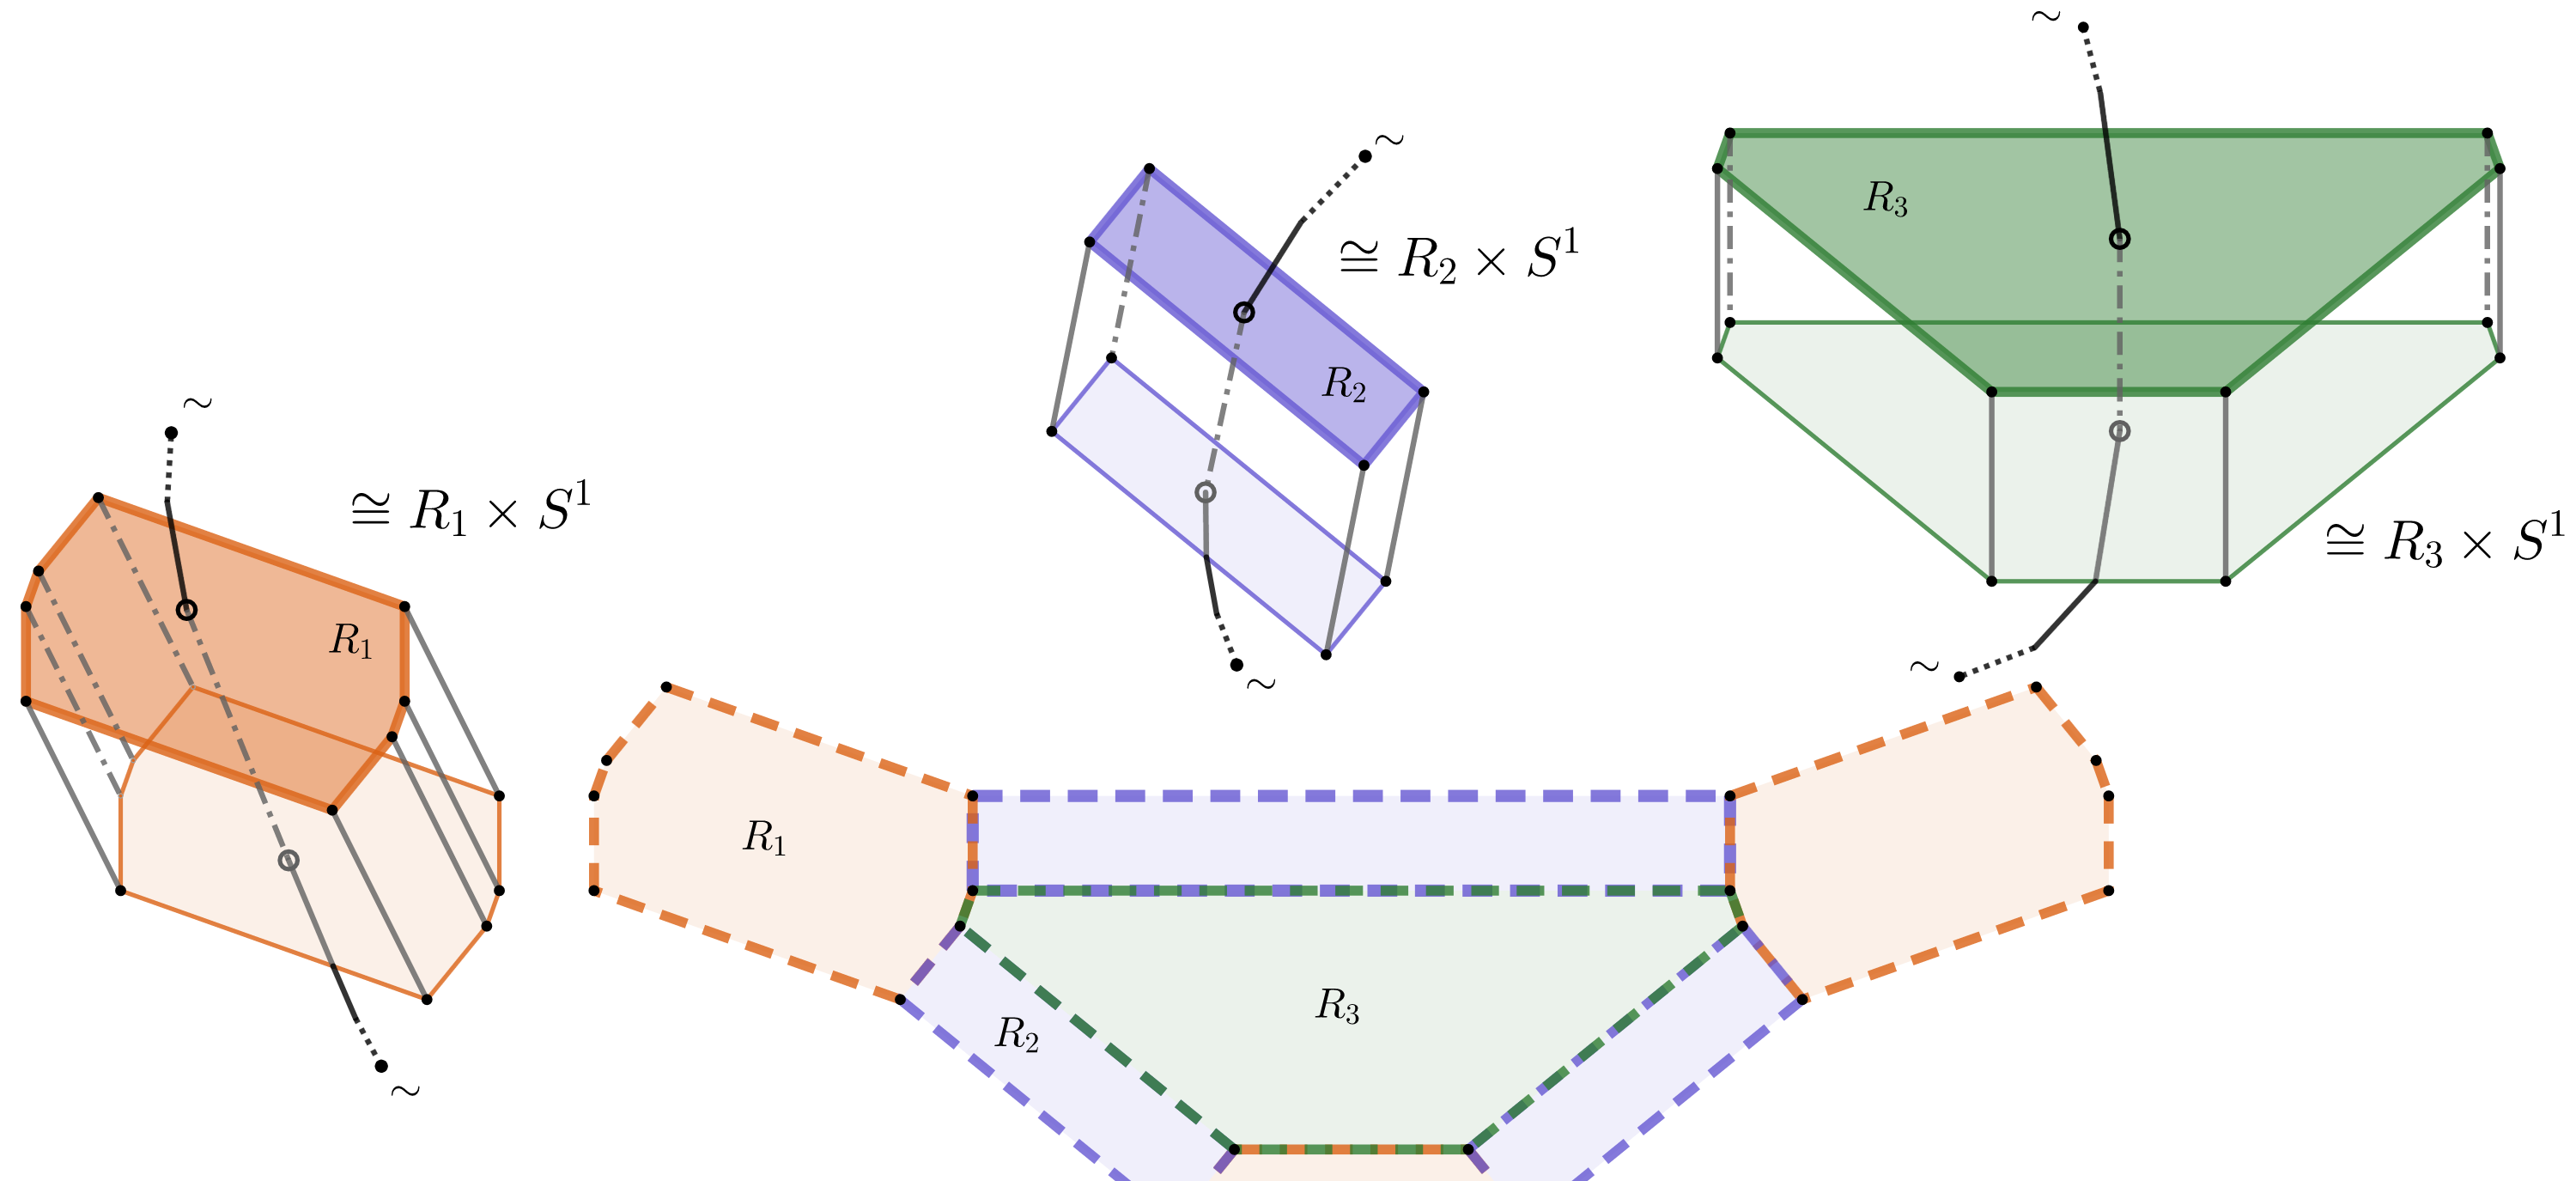
\includegraphics{figures/regular-blocks.png}
		\caption{
			\textbf{Regular blocks.}
			Three types of regular blocks.
			These are found as regular fibers over face, edge, and vertex regions.
		}
		\label{fig:regular-blocks}
	\end{figure}
	
	\textbf{Part 2:}
	Let $B$ be a definite or indefinite block over the region $R$.
	$R$ is a subset of the plane homeomorphic to $D^2$ with an arc $\gamma_s \subset X_f$ of singular values running from one of its edges to another.
	Let $\gamma_t$ be a second simple arc that crosses $\gamma_s$ transversely, and consider the cross-sectional surface obtained by $f\inv(\gamma_t)$.
	Figure \ref{fig:codim-1-surfaces} illustrates the possible surfaces containing the singular fiber over $x=\gamma_s\cap\gamma_t$.
	
	\begin{figure}[h]
		\centering
		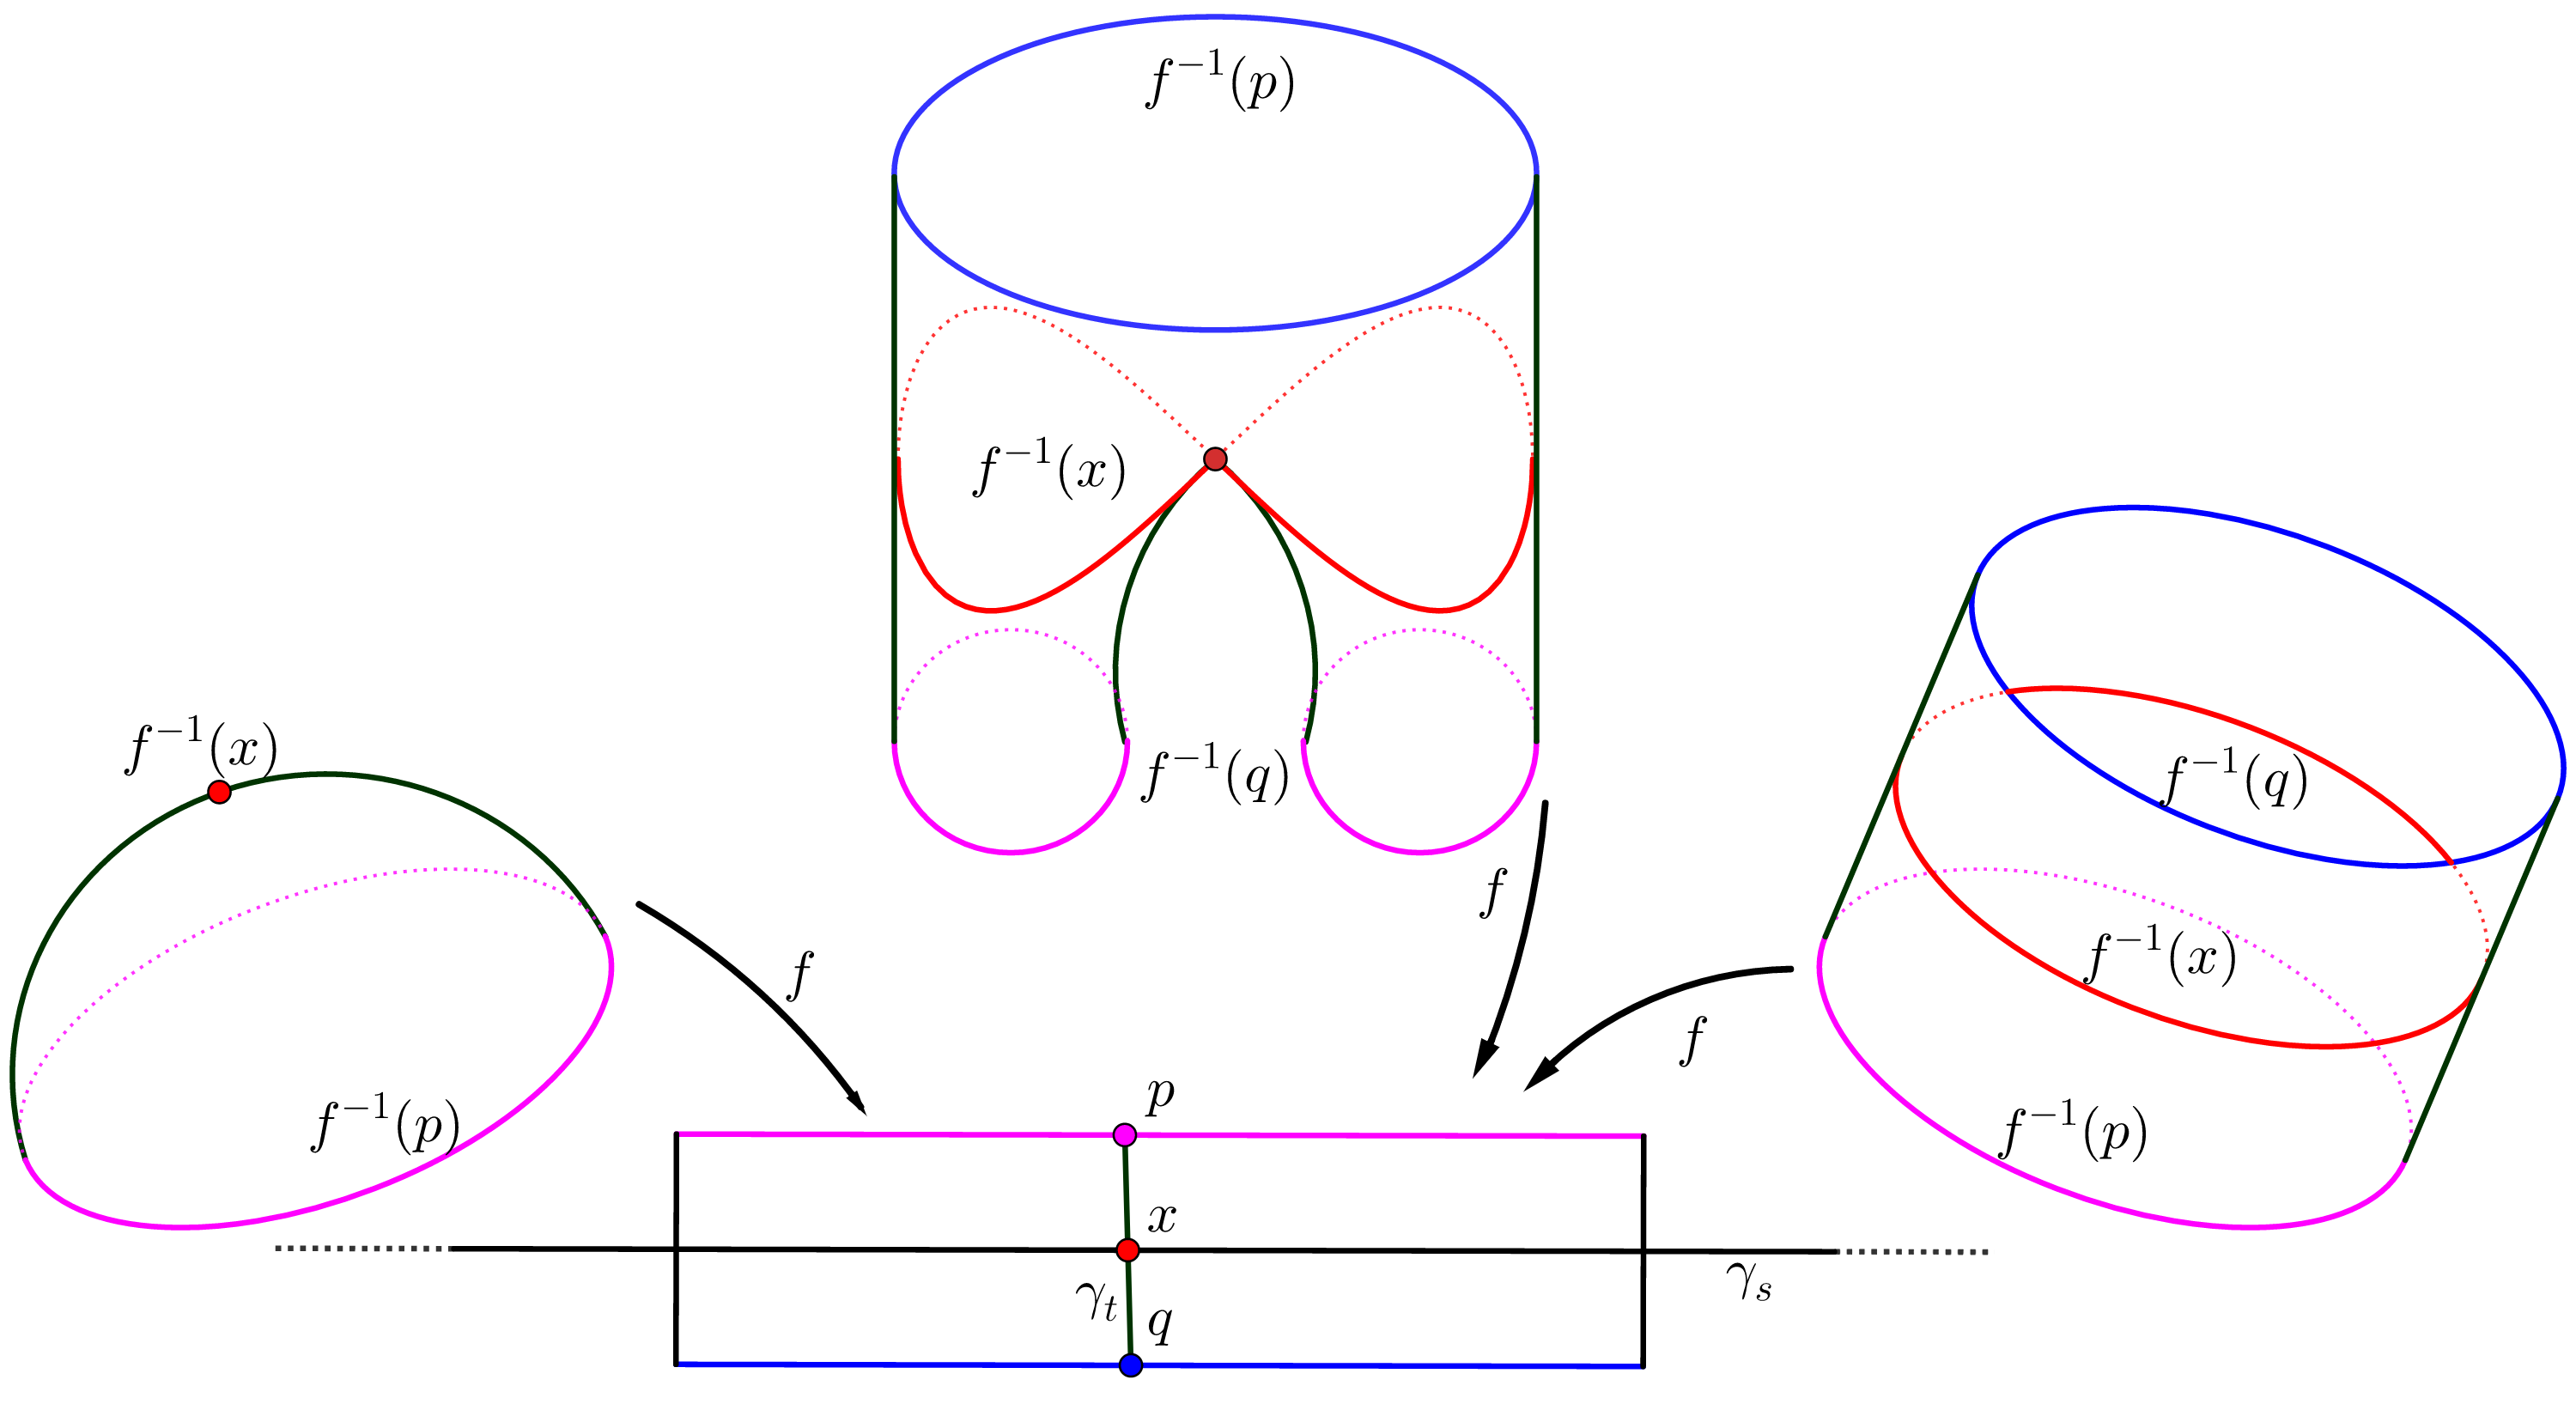
\includegraphics[width=\textwidth]{figures/codim-1-surfaces.png}
		\caption{
			\textbf{Surfaces over codimension 1 singularities.}
			$\gamma_s$ is an arc of singular values and $\gamma_t$ is an arc with endpoints $\pd\gamma_t = \{p,q\}$ that intersects $\gamma_s$ transversely at $x=\gamma_s\cap\gamma_t$.
			The three surfaces shown are the three possible cross-sectional surfaces that can project through $f$ over $\gamma_t$.
		}
		\label{fig:codim-1-surfaces}
	\end{figure}
	
	This cross section is general, so we fit a tubular neighbourhood $\nu(\gamma_s)$ about $\gamma_s$ in $R$ to obtain a bundle structure for $f\inv(\nu(\gamma_s))$ whose fiber is one of the cross-sectional surfaces (a disk or a pair-of-pants) and whose base is the arc $\gamma_s$, i.e. an interval.
	The interval is contractible, so $f\inv(\nu(\gamma_s))$ is homeomorphic to $\Sigma\times\Ilit$ for $\Sigma$ a disk or a pair-of-pants surface.
	Away from $\nu(\gamma_s)$, $R$ consists entirely of regular values so we obtain solid tori (cf. Part 1) that extend the $\Sigma\times\Ilit$ structure as seen in Figure \ref{fig:codim-1-blocks}.
		
	\begin{figure}[h]
		\centering
		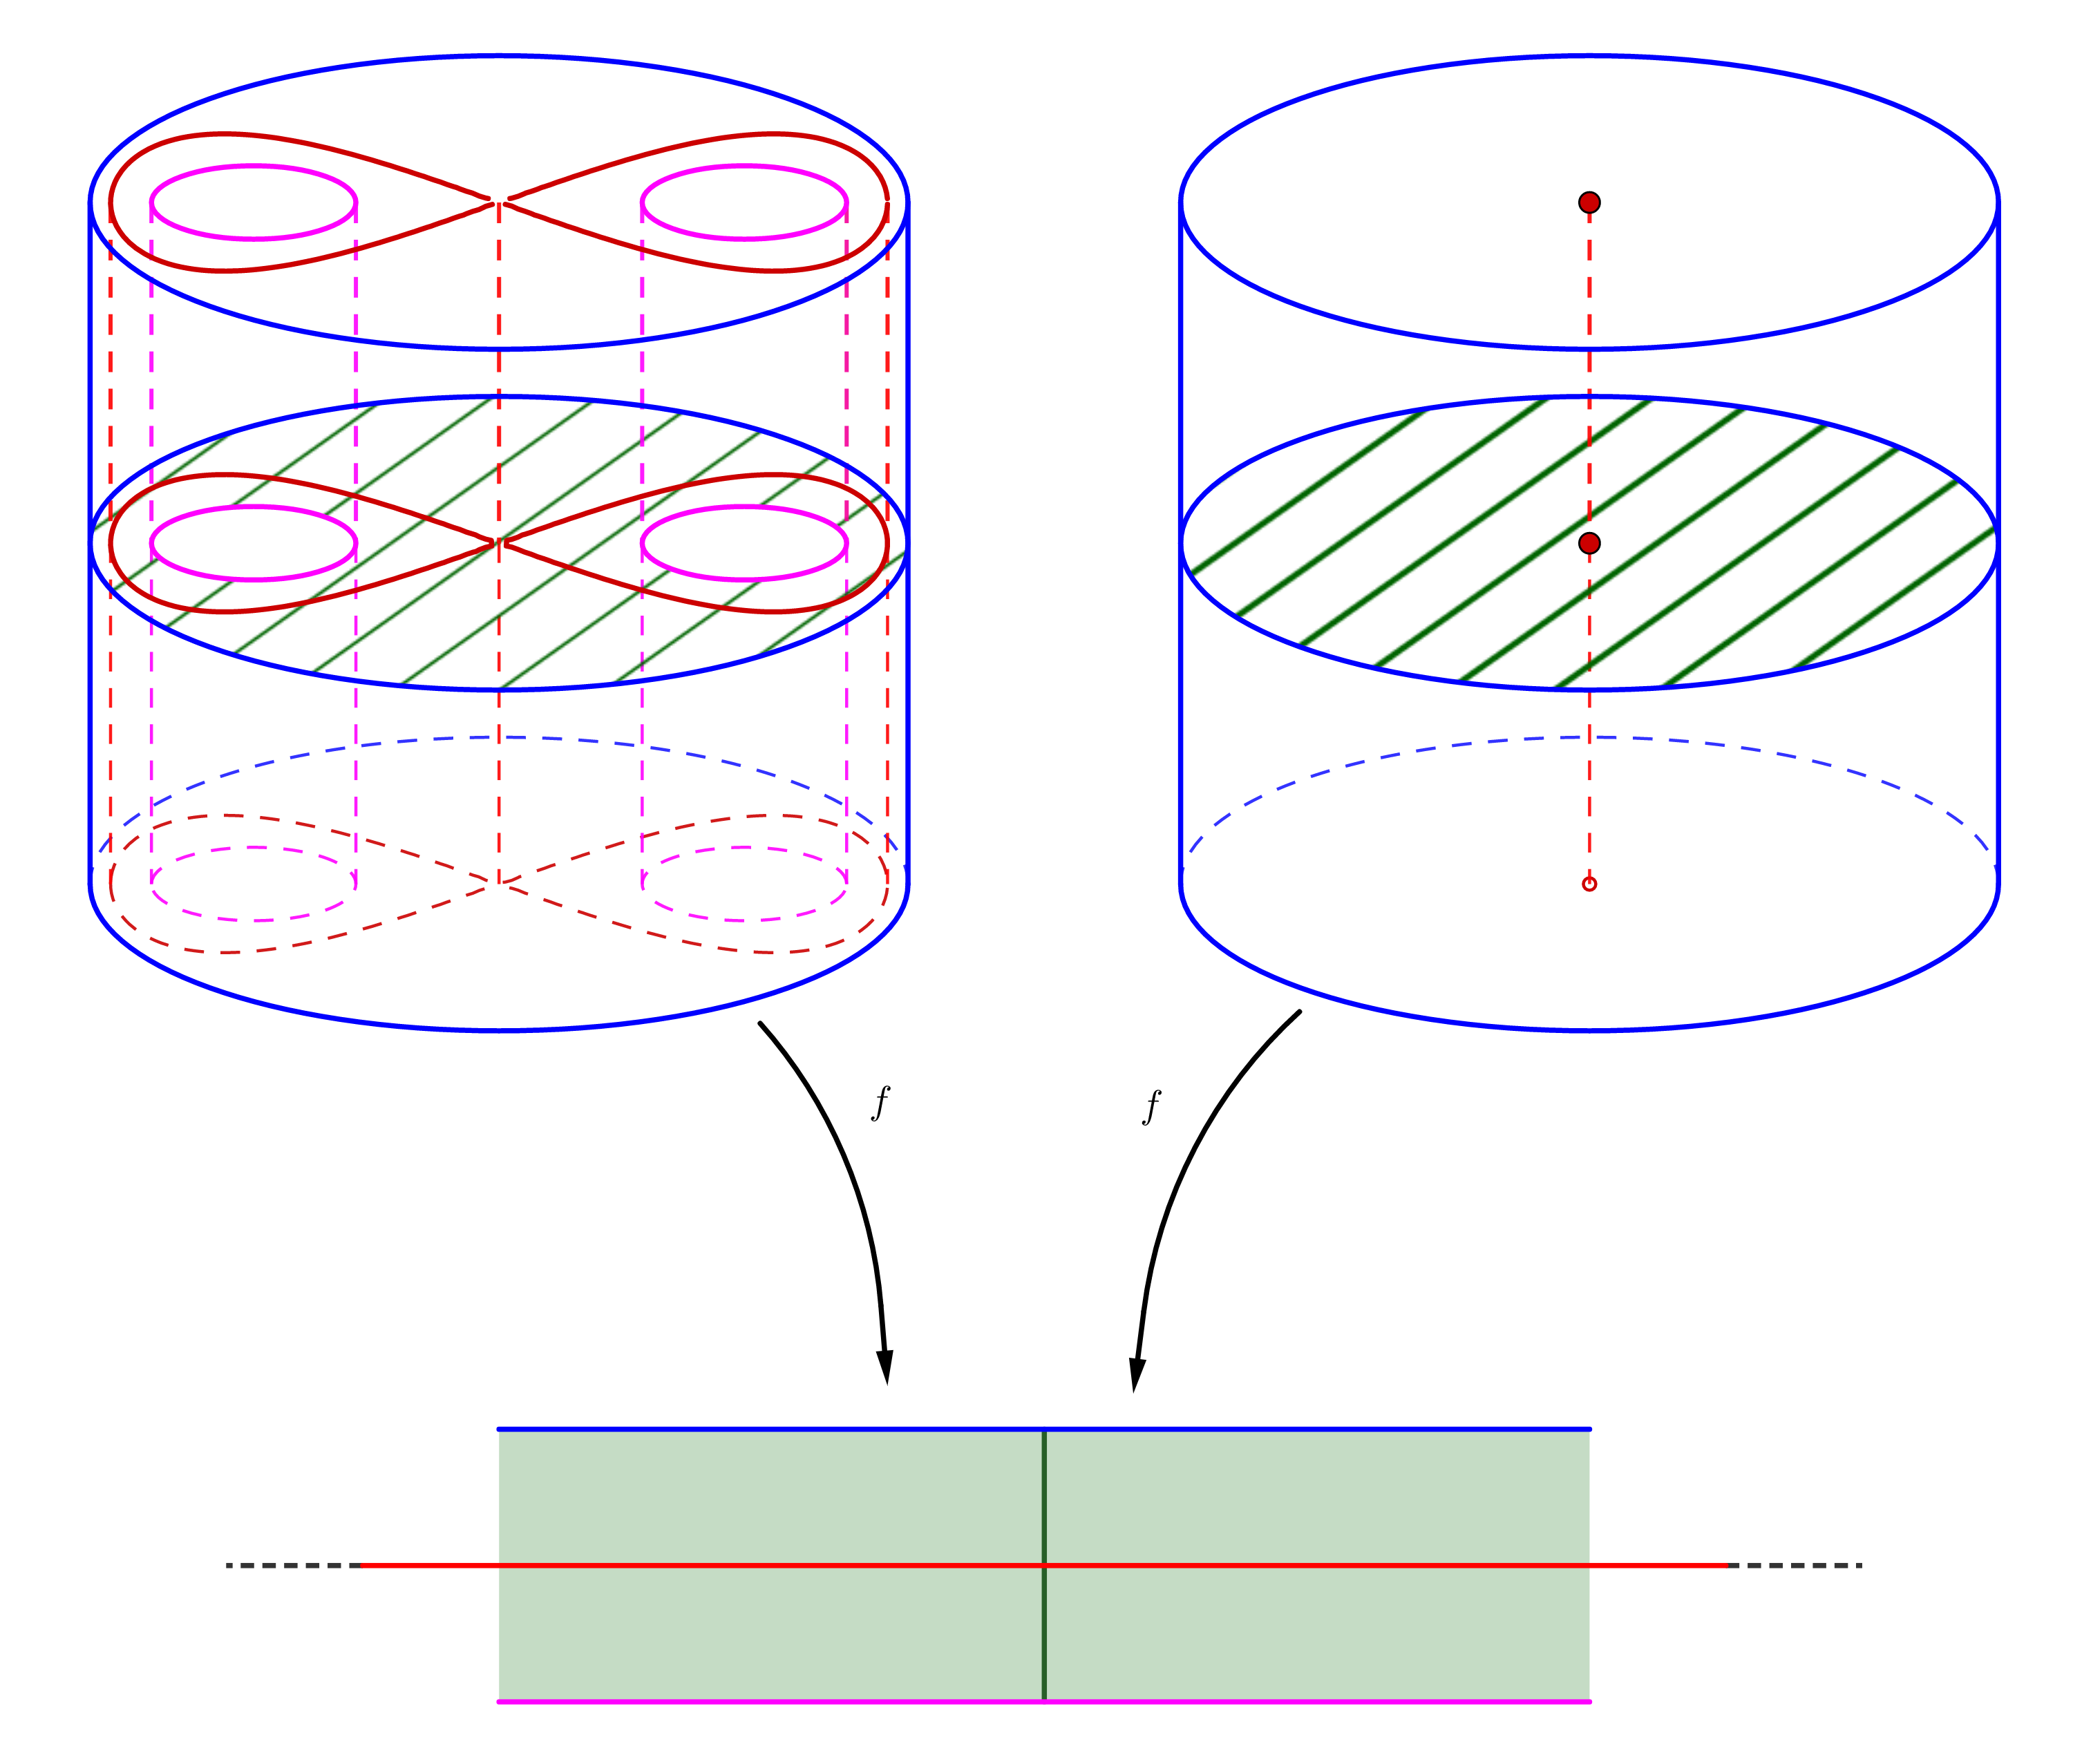
\includegraphics[width=\textwidth]{figures/codim-1-blocks.png}
		\caption{
			\textbf{Definite and indefinite blocks.}
			The blocks containing sections of definite and indefinite folds that project over codimension 1 singular values.
			These are found as singular fibers over edge and vertex regions.
		}
		\label{fig:codim-1-blocks}
	\end{figure}

	As with Part 1, the homeomorphism described is stratified by ensuring the strata of $B$ are mapped to the strata of $\Sigma \times \Ilit$, where the stratification of $\Sigma \times \Ilit$ is defined by the manifold with corners structure induced by the product topology.
	
	\textbf{Part 3:}	
	Let $B$ be an interactive block over the region $R$.
	Interactive blocks occur over octagonal vertex regions where the singular fiber above the region's codimension 2 singularity is connected, so we investigate these fibers.
	The codimension 2 singular value lies at the intersection of a pair of arcs of codimension 1 singular values.
	Call the arcs $\gamma_1$ and $\gamma_2$, let $x = \gamma_1\cap \gamma_2$, and denote the interactive singular fiber over $x$ by $B_x = B\cap f\inv(x) = \{b\in B\:|\:f(b)=x\}$.
	Our method of investigation begins by examining the possible resolutions of $B_x$ and combining those resolutions to form a genus 3 surface.
	 
	Figure \ref{fig:codim-2-interactive-fiber-1} demonstrates resolutions of the singular points of $B_x$ when $B_x$ has the first interactive singular fiber form presented in Figure \ref{fig:saeki-fibers}.
	We first note that all of the displayed fibers have inherited an orientation from $M$.
	This forces fiber resolution to be unambiguous, and allows us to identify fibers when forming the surface shown in Figure \ref{fig:codim-2-surface-1}.
	
	\begin{figure}[h]
		\centering
		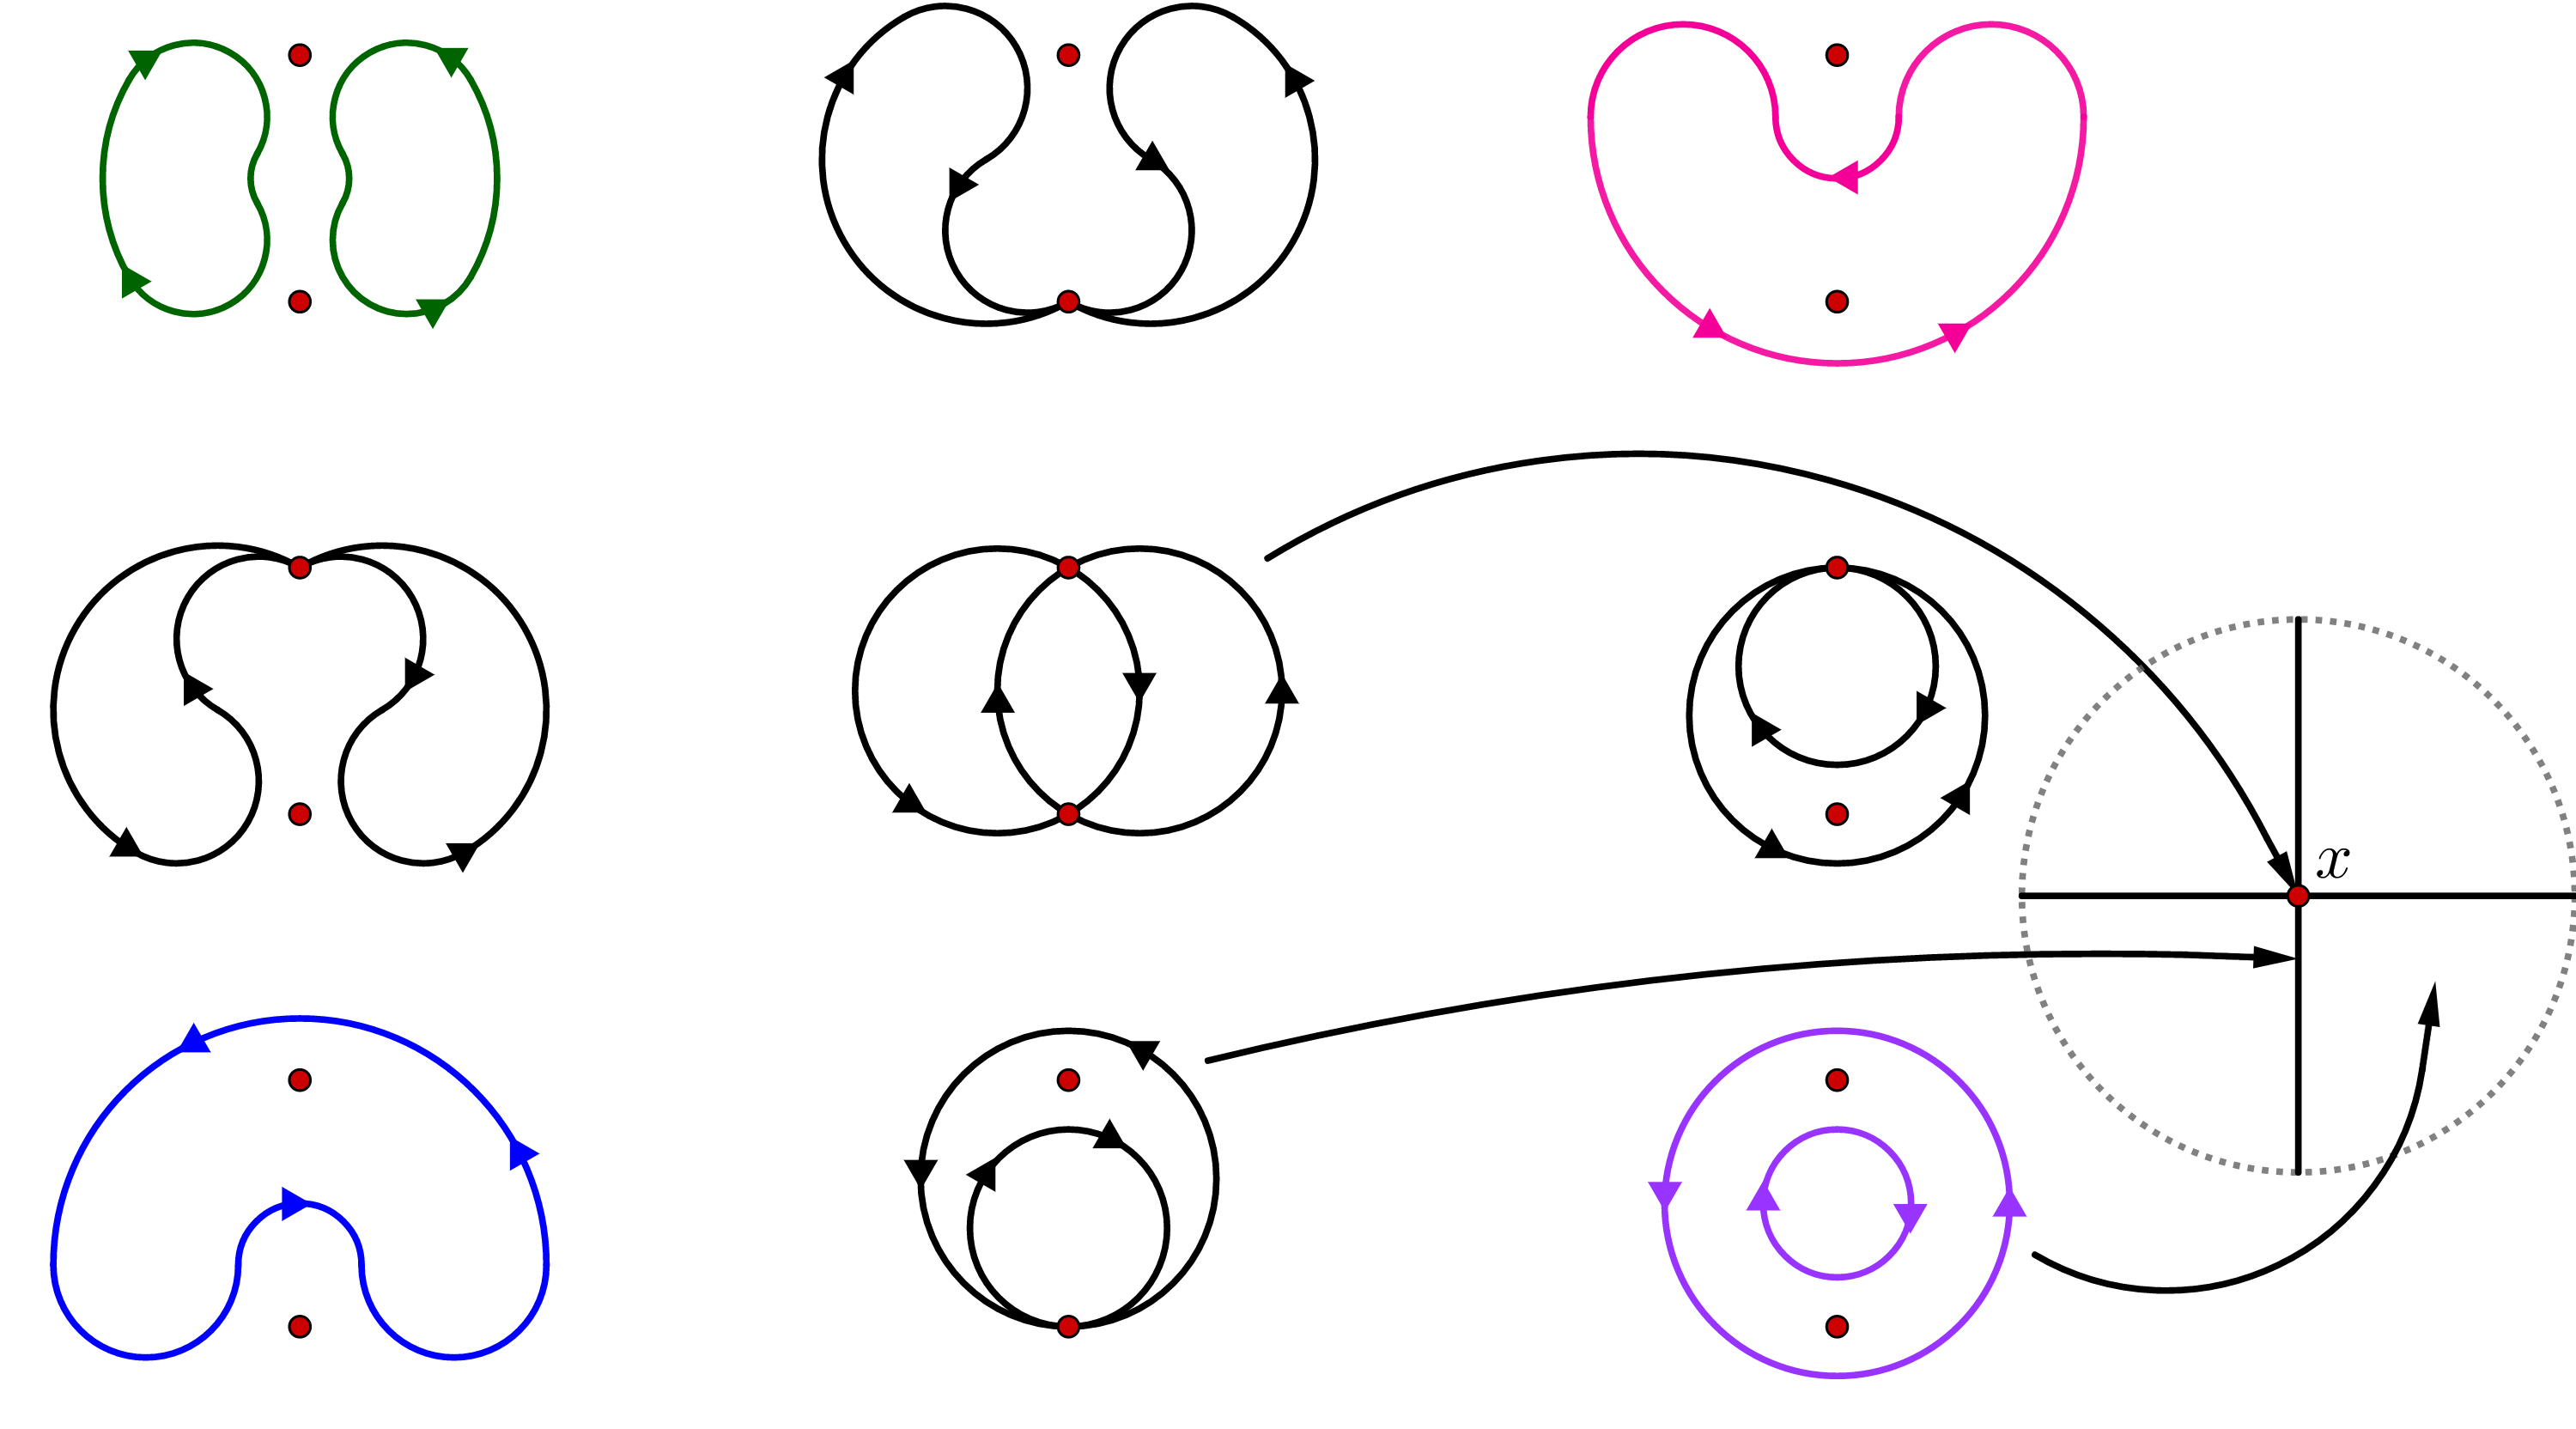
\includegraphics[width=\textwidth]{figures/codim-2-interactive-fiber-1.png}
		\caption{
			\textbf{Resolutions of the singular points in the first interactive fiber.}
			The singular fiber inside of $B_x$ and its possible resolutions over nearby codimension 1 singular values and regular values.
			The fibers inherit orientation from $M$, and this illustration is presented without loss of generality.
			This figure is modeled after Figure 18 from \cite{CostThur08}.
		}
		\label{fig:codim-2-interactive-fiber-1}
	\end{figure}

	\begin{figure}[h]
	\centering
	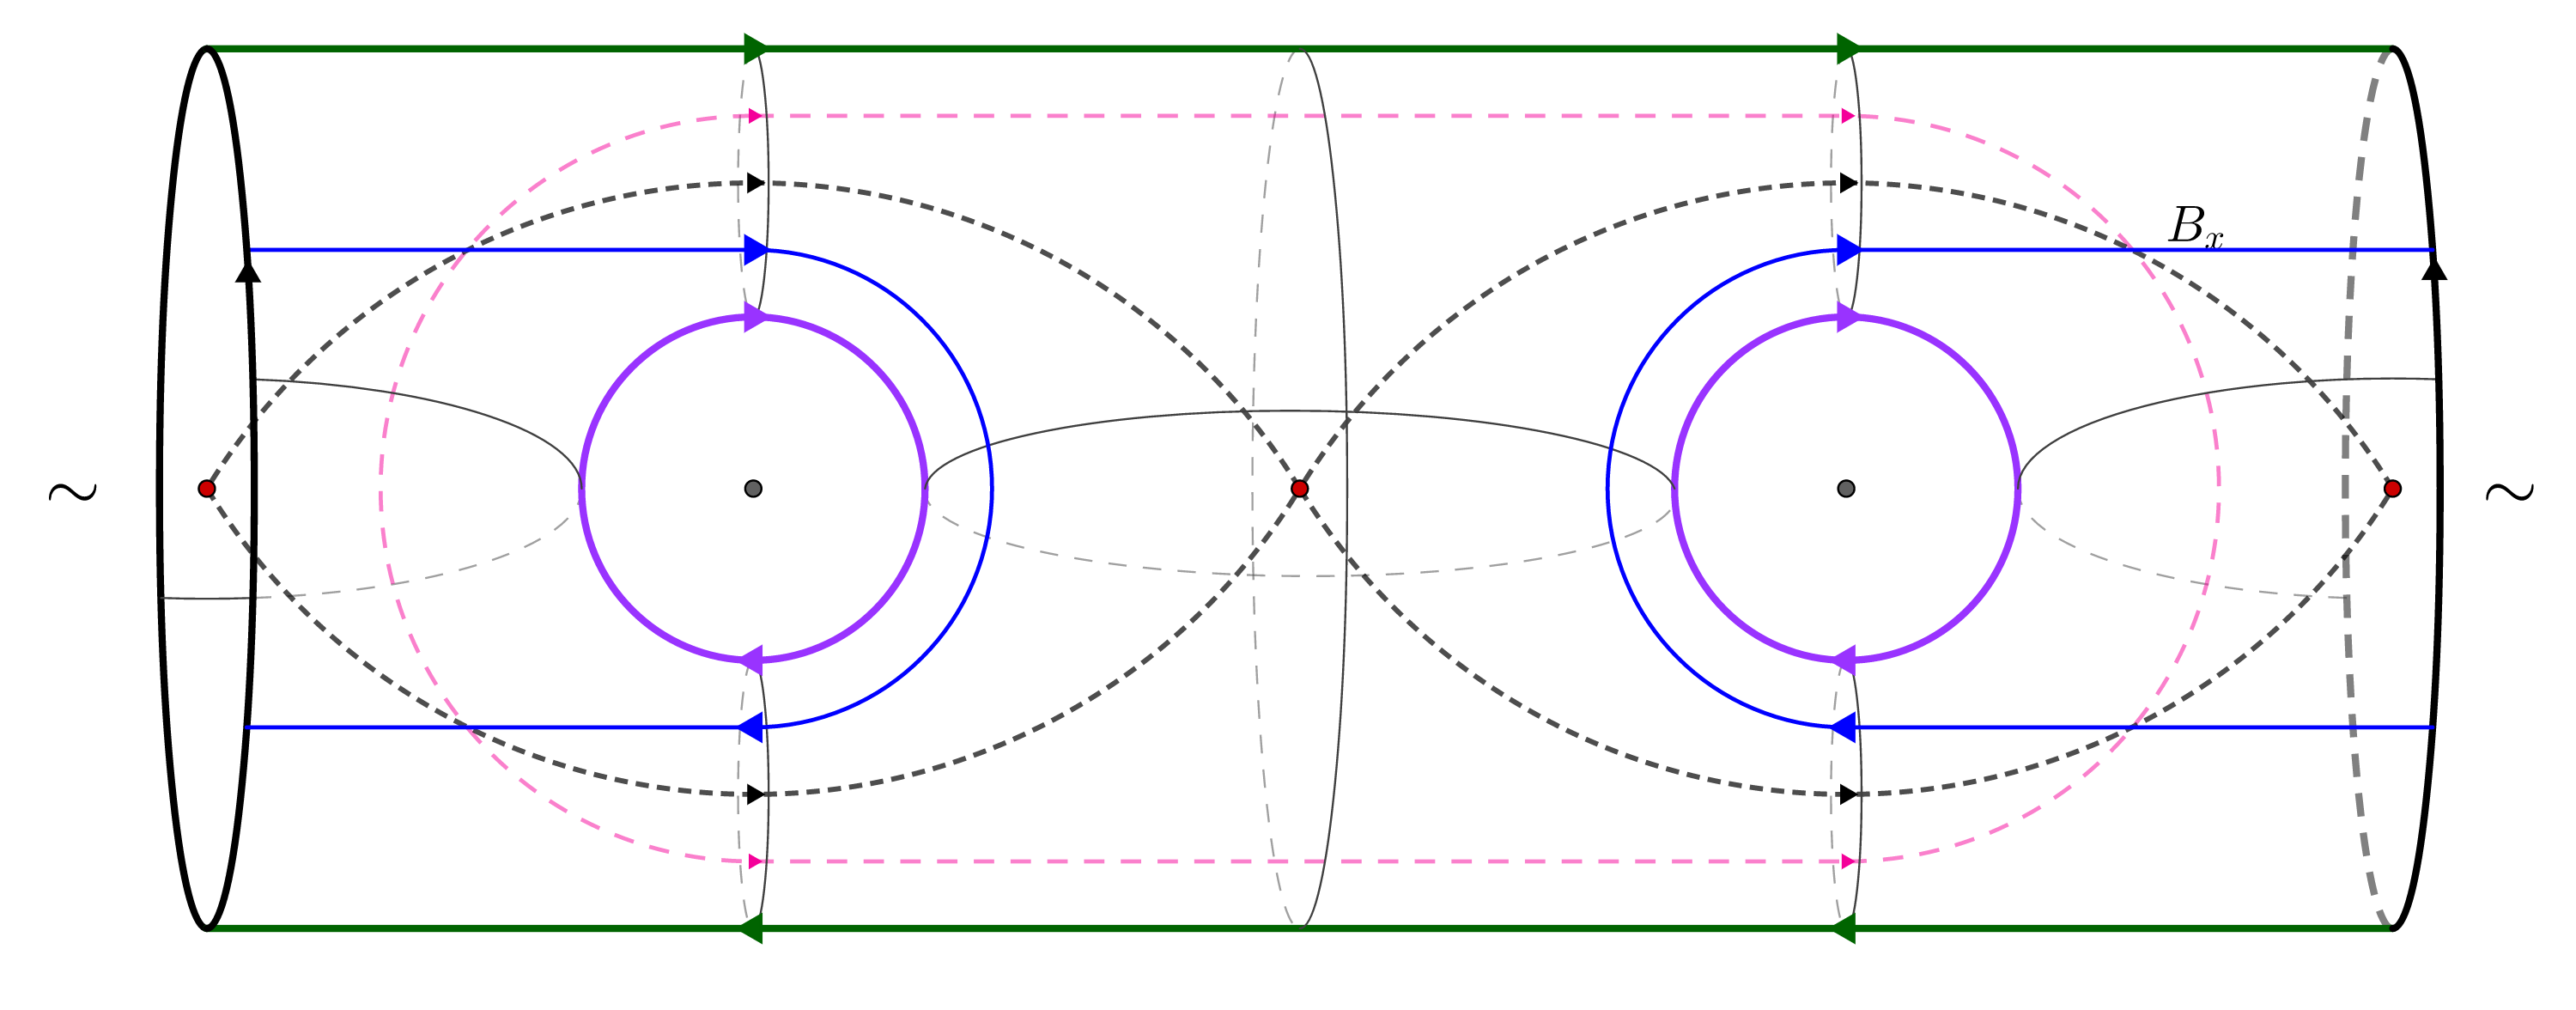
\includegraphics[width=\textwidth]{figures/codim-2-surface-1.png}
	\caption{
		\textbf{Surface $\Sigma$ near the first interactive fiber that projects over $\pd\bar\nu(x)$.}
		The surface and $B_x$ are presented as embedded in $S^3$, where $H(B_x)$ is the genus-3 (3,1)--handlebody on the `inside' of $\Sigma$ in $S^3$.
	}
	\label{fig:codim-2-surface-1}
	\end{figure}

	We form the surface shown in Figure \ref{fig:codim-2-surface-1} by gluing together surfaces that project over simple arcs transversing the codimension 1 singular values.
	Gluing is performed over the boundary circles of these surfaces, and is prescribed by the resolutions in Figure \ref{fig:codim-2-interactive-fiber-1}.
	The transverse preimage containing the top row of fibers in Figure \ref{fig:codim-2-interactive-fiber-1} is a pair of pants with two green 'cuffs' (top left) and a pink 'waist' (top right).
	The preimage containing the right column is a pair of pants with a pink waist (top right) and two purple cuffs (bottom right).
	The first gluing that helps realize the surface in Figure \ref{fig:codim-2-surface-1} is of the 'top' transverse preimage surface with the 'right' transverse preimage surface over their shared pink waist.
	The bottom row and left column each also produce single pairs of pants, and we continue the gluing: purple cuffs to purple cuffs from right to bottom, blue waist to blue waist from bottom to left, then green cuffs to green cuffs from left to top.
	Figure \ref{fig:codim-2-surface-1} depicts the result of this gluing.


	
	The surface $\Sigma$ in Figure \ref{fig:codim-2-surface-1} is the boundary of $H(B_x)$, a regular neighbourhood of $B_x$ in $M$, i.e. a genus-3 (3,1)--handlebody inside of $M$.
	$H(B_x)$ projects through $f$ over $\bar\nu(x)$, a closed tubular neighbourhood of $x$, and $\Sigma$ projects over $\pd(\bar\nu(x))$.
	
	Figure \ref{fig:codim-2-surface-1} presents $\Sigma$ and $B_x$ as objects embedded in $S^3$, where $\Sigma$ bounds genus-3 (3-1)--handlebodies on both sides.
	We take the `inside' component of $S^3\setminus\Sigma$ (i.e. the component containing $B_x$) to be $H(B_x)$.
	
	Outside of $\bar\nu(x)$ we use the investigations from Parts 1 and 2 of this proof. The rest of $R$, $f\inv(R\setminus\bar\nu(x))$, has the structure of a $\Sigma$-bundle over the interval, and the bundle extends $H(B_x)$ to the boundary of $R$, preserving the structure as a genus-3 (3,1)--handlebody.
	We conclude that $B$ is homeomorphic to a genus-3 (3,1)--handlebody.
	
		\begin{figure}[h]
		\centering
		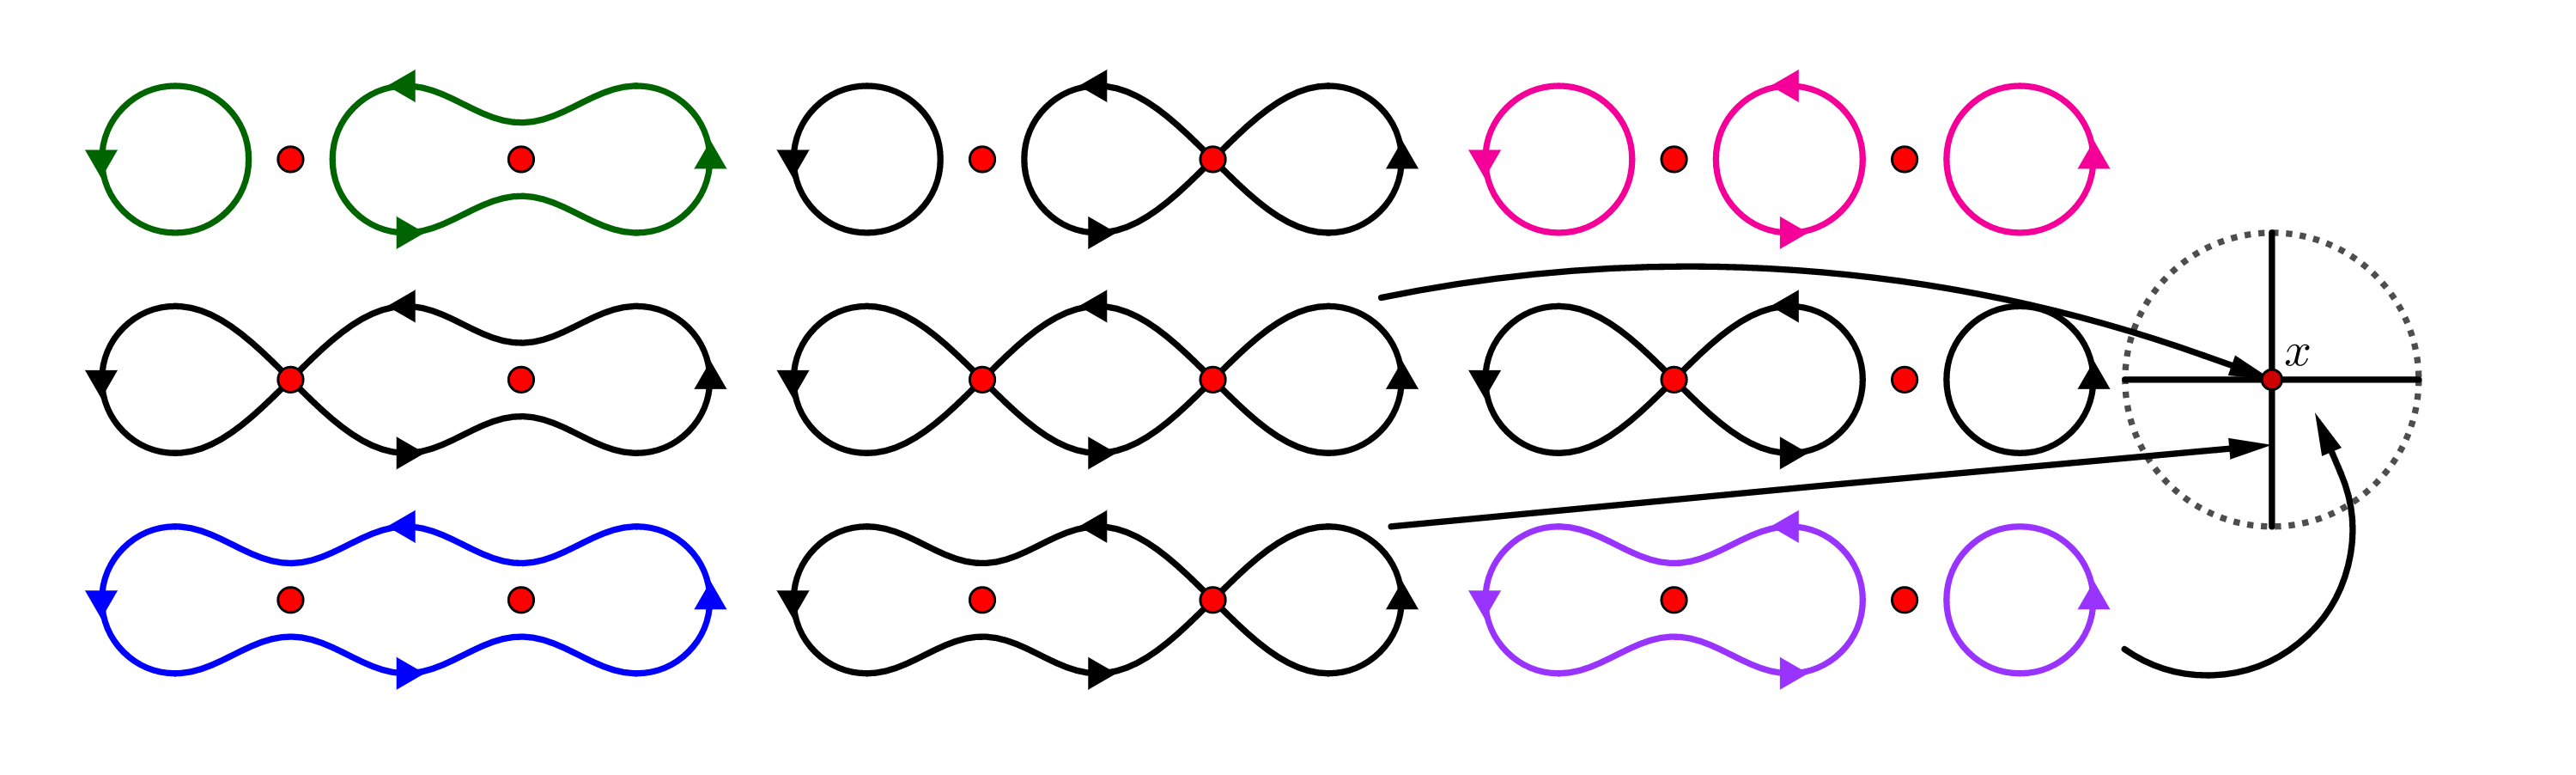
\includegraphics[width=\textwidth]{figures/codim-2-interactive-fiber-2.png}
		\caption{
			\textbf{Resolutions of the singular points in the second interactive fiber.}
			The singular fiber inside of $B_x$ and its possible resolutions over nearby codimension 1 singular values and regular values.
			The fibers inherit orientation from $M$, and this illustration is presented without loss of generality.
			his figure is modeled after Figure 16 from \cite{CostThur08}.
		}
		\label{fig:codim-2-interactive-fiber-2}
	\end{figure}
	
	\begin{figure}[h]
		\centering
		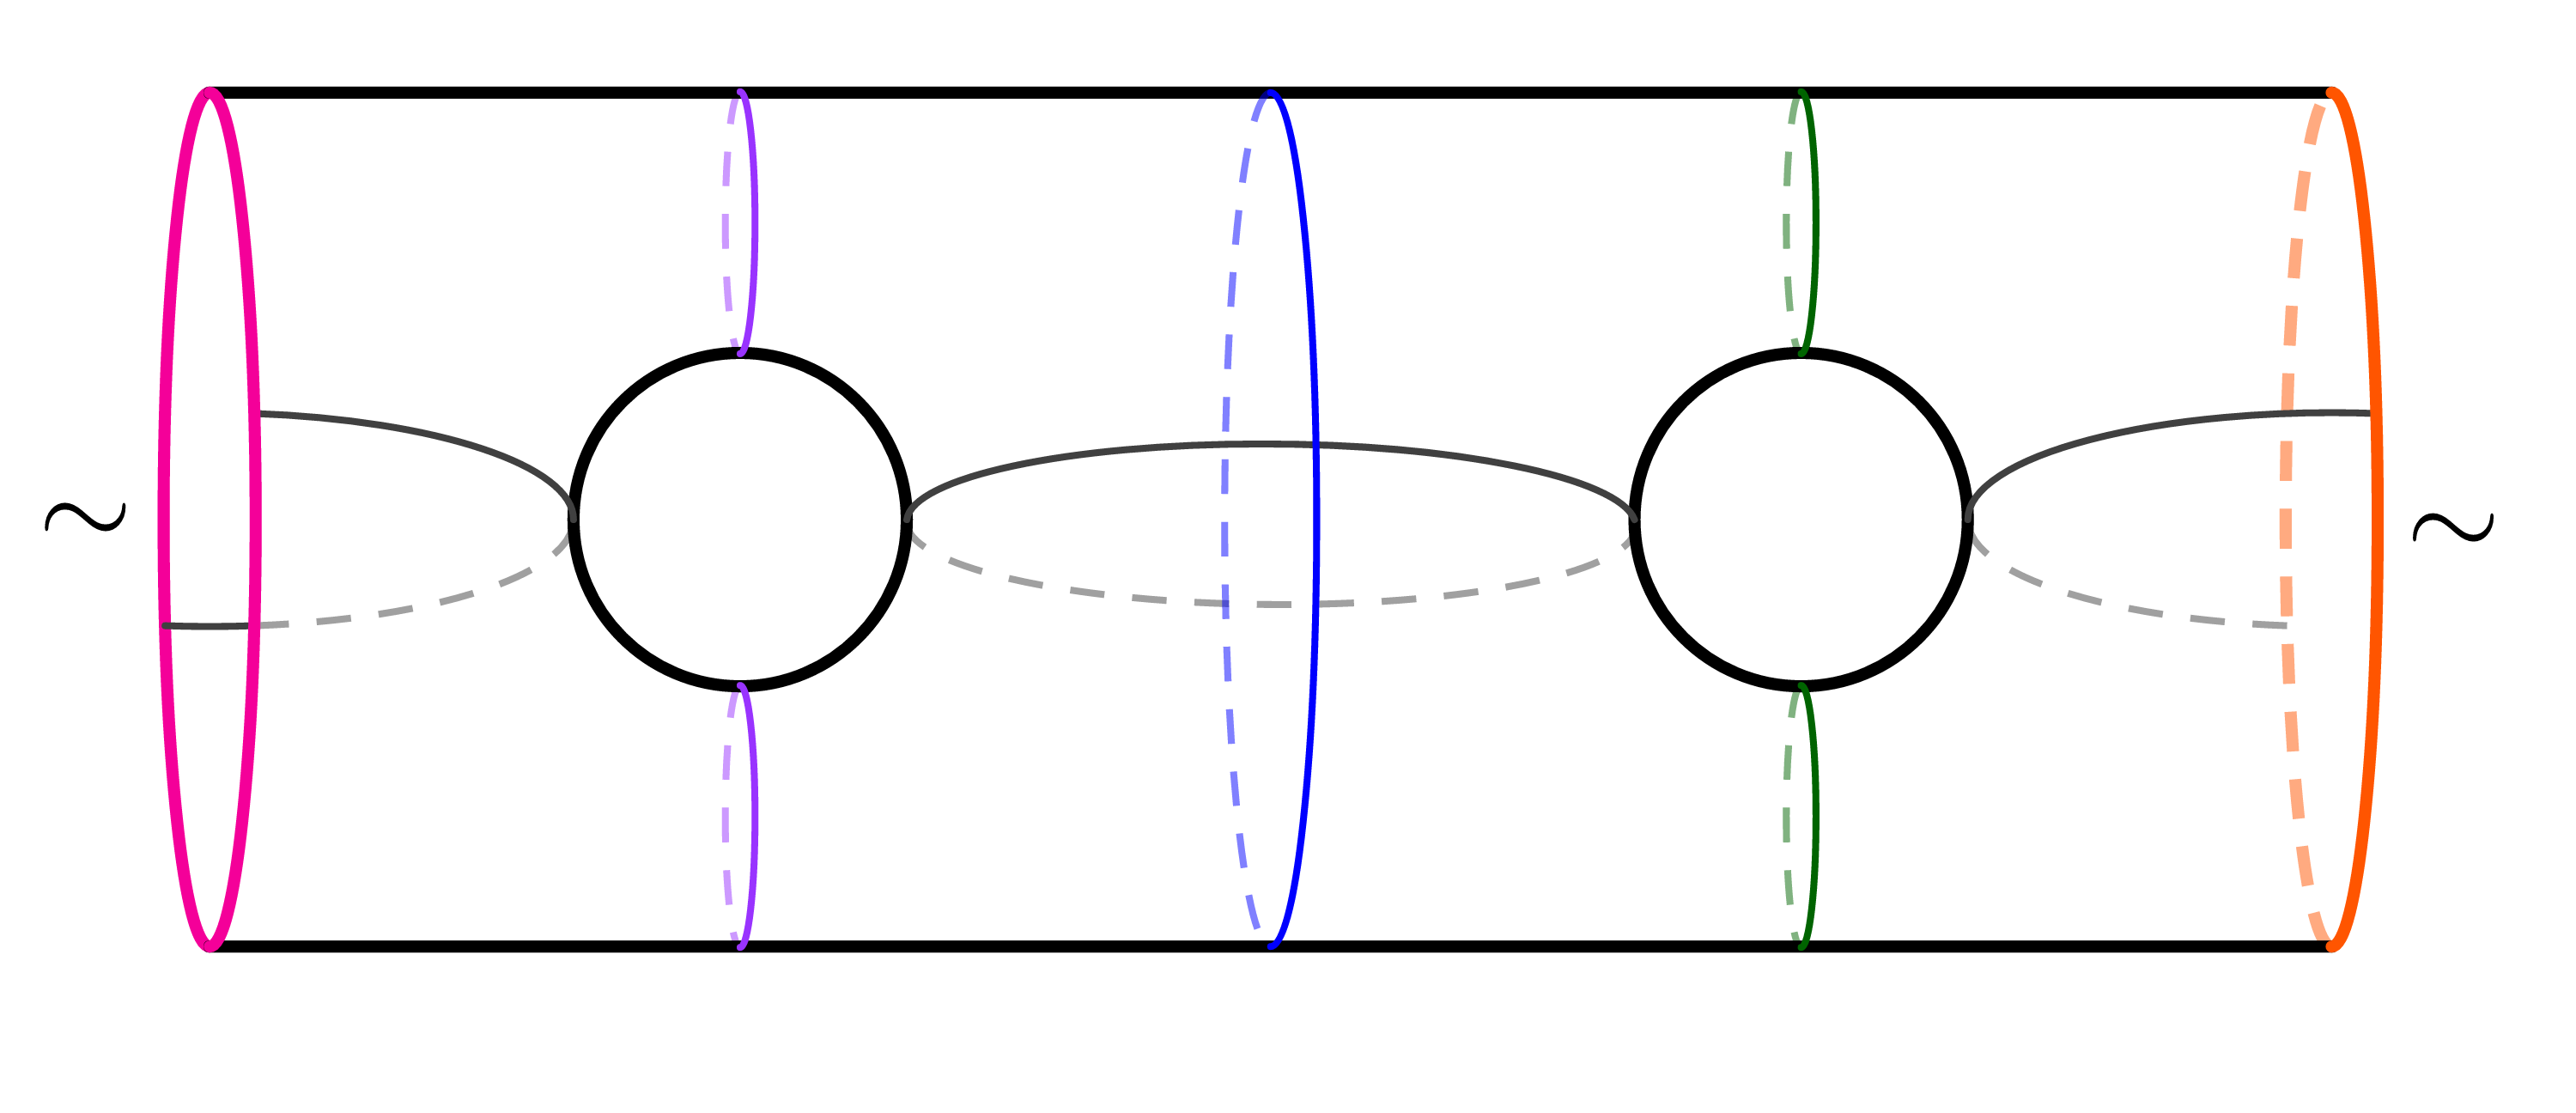
\includegraphics[width=\textwidth]{figures/codim-2-surface-2.png}
		\caption{
			\textbf{Surface $\Sigma$ near the second interactive fiber that projects over $\pd\bar\nu(x)$.}
			The surface and $B_x$ are presented as embedded in $S^3$, where $H(B_x)$ is the genus-3 (3,1)--handlebody on the `outside' of $\Sigma$ in $S^3$.
		}
		\label{fig:codim-2-surface-2}
	\end{figure}

	An identical argument is made when $B_x$ has the second interactive singular fiber form, using Figures \ref{fig:codim-2-interactive-fiber-2} and \ref{fig:codim-2-surface-2} in place of Figures \ref{fig:codim-2-interactive-fiber-1} and \ref{fig:codim-2-surface-1} respectively.
	In this case the surfaces recovered as transversal preimages are:
	{\renewcommand\labelitemi{}
	\begin{itemize}
		\item \textbf{Left:} a pair of pants with blue waist and green cuffs
		\item \textbf{Top:} the disjoint union of a pair of pants with green waist and pink cuffs with an annulus with one green boundary circle and one pink boundary component
		\item \textbf{Right:} the disjoint union of a pair of pants with purple waist and pink cuffs with an annulus with one purple boundary circle and one pink boundary component
		\item \textbf{Bottom:} a pair of pants with blue waist and purple cuffs
	\end{itemize}
	}
	


%	Figure \ref{fig:codim-2-blocks} displays both possible interactive block structures, highlighting their boundaries.
%	The figure explains that the blocks are the handlebodies on the `outside' of the illustrated surfaces.
%	This is specifically to aid visualization of the effects of 2-- and 3--handle attachment in the next two sections, as the result of these attachments will fill the genus-3 (3,1)--handlebody on the `inside' of the illustrated surface.

%	\begin{figure}[h!]
%%		HAND DRAW THIS FIGURE
%	\caption{
%		\textbf{Possible interactive block structures embedded in $S^3$.}
%		Interactive blocks with indicated boundary stratification induced by $f\inv \pd R$.
%		Blocks are embedded in $S^3$, outside of the illustrated stratified boundary surfaces.
%	}
%	\label{fig:codim-2-blocks}
%	\end{figure}
\end{proof}

A smooth map $f$ satisfying the stratification conditions of Section \ref{section:smooth-projection} induces a decomposition on $\RR$ and a stratification of $M$.
It is important to note here that the restrictions on $f$ can induce a wide variety of possible stratifications of $M$, highlighting the variability of the resulting 4--manifold.
We end this section with a lemma that guarantees the stratified 2--handle attachments of the next section can be made over our face blocks in any order, hence we can assume all attachments occur simultaneously.


\begin{lem}
	Let $M$ be a 3--manifold with stratification induced as in Theorem \ref{thm:block-structure}.
	Then blocks of the same type (i.e. face, edge, vertex) are disjoint.
\end{lem}

\begin{proof}
	The fibers above a given region are disjoint, so the blocks above that region are disjoint.
	Regions of the same type are disjoint, hence blocks that are fibers above differing regions are also disjoint.
\end{proof}


